%--------------------------------------------------------------------
\medskip
\subsection{Análisis del modelo}
En esta última sección se expone un análisis para probar el modelo multidimensional implementado en la sección \ref{11}, haciendo uso de los visores OLAP proporcionados en la máquina virtual del módulo. \\

Este análisis consiste en saber la cantidad de encuestas realizadas entre los días 1 (sábado) y 5 (miércoles) del mes de febrero del año 2014, así como el total de los resultados y el resultado máximo y mínimo obtenido por día. Gráficamente el resultado se muestra en la Figura \ref{analisis}, donde se puede observar que el número total de encuestas es menor durante el fin de semana (días 1 y 2), aunque sus resultados suelen ser mejores que los obtenidos en el resto de la semana (si nos fijamos, el resultado mínimo que se obtuvo el sábado día 1, fue entre 0.5 y 0.6, lo que nos puede indicar que los sábados se obtienen mejores resultados). También comentar que durante esos días, hubo al menos una encuesta que obtuvo un resultado cercano (incluso llegando) a 1 a la vez que también hubo encuestas que tuvieron como resultado 0.

\begin{figure}[!th]
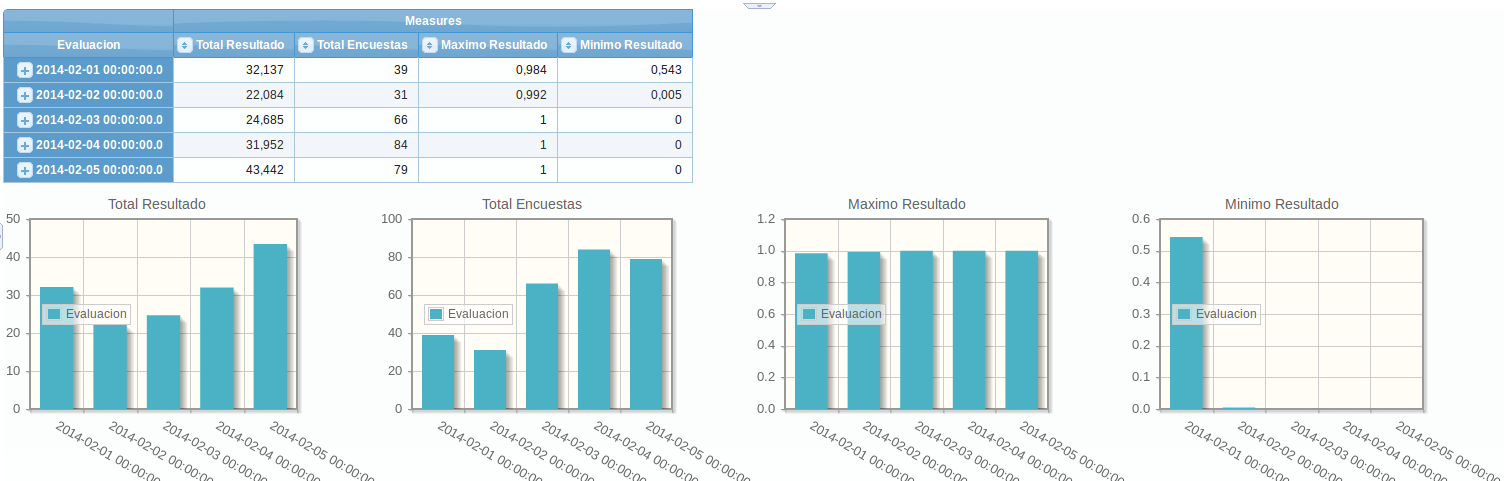
\includegraphics[scale=0.35]{analisis.png}
\centering
\caption{Análisis del modelo multidimensional utilizando visores OLAP.}
\label{analisis}
\end{figure}

Lógicamente, este análisis es muy básico, ya que era para probar el modelo multidimensional implementado. Las observaciones que se han obtenido y comentado anteriormente, no dejan de ser eso, observaciones, y que se deberían de confirmar analizando más profundamente el modelo y ver si lo que se ha comentado es real o no.
